% \input{"//iab.baintern.de/Dfs/017/Ablagen/D01700-Info-Board/06_WMK/Corporate Design/Folienvorlagen/TeX-Folienformat.tex"}
\input{"/Users/jonathanlatner/Google Drive/My Drive/IAB/latex/TeX-Folienformat.tex"}


\documentclass[t,8pt,utfx8]{beamer}
\usepackage{booktabs}
\usepackage{setspace}
\usepackage{parskip}
\setbeamertemplate{caption}[numbered]
\newcommand{\sprache}{\englisch}
\renewcommand{\thesubsection}{\alph{subsection})}

\newcommand{\btVFill}{\vskip0pt plus 1filll}

\title[Balancing data utility and privacy]{Balancing data utility and privacy: Evaluating computer science and statistical approaches to creating synthetic data}
\subtitle{Statistische Woche\\
        Dortmund, Deutschland \\
         11. September, 2023}

\author{Jonathan Latner, PhD \newline Prof. Dr. Jörg Drechsler}

\newcounter{noauthorlines}
\setcounter{noauthorlines}{2} % Wert für 2 Autoren über 2 Zeilen. Ggf. anpassen

% %%%%%%%%%%%%%%
% Ende Anpassung
% %%%%%%%%%%%%%%

% \input{"//iab.baintern.de/Dfs/017/Ablagen/D01700-Info-Board/06_WMK/Corporate Design/Folienvorlagen/TeX-Folienformatierung_CD_2019"}
\input{"/Users/jonathanlatner/Google Drive/My Drive/IAB/latex/TeX-Folienformatierung_CD_2019"}

% Modify the section in toc template to enumerate
\setbeamertemplate{section in toc}{%
    \inserttocsectionnumber.~\inserttocsection\par
}

% use for subsections
\setbeamertemplate{subsection in toc}{}
% \setbeamertemplate{subsection in toc}{%
%     \setlength{\parskip}{1mm}
%     %     \hskip2mm -- \hskip1mm\inserttocsubsection\par
% }

\titlegraphic{\includegraphics[width=2cm]{/Users/jonathanlatner/Google Drive/My Drive/IAB/latex/CD 2019/aniged.png}}

\begin{document}


\section{Introduction}\label{sec_intro}
\frame[plain]{\titlepage}

\begin{spacing}{1.25}

%Table of contents
\begin{frame}
\frametitle{Sections}
\vskip6mm
\setlength{\leftskip}{0.5mm}
\setlength{\parskip}{5mm}
\begin{NoHyper}
        \tableofcontents
\end{NoHyper}
\end{frame}

\frame[c]{\frametitle{}
\centering
Section \ref{sec_intro}: Introduction
}



\frame{\frametitle{Overview}
\begin{itemize}
    \item {\bf Definition:} Synthetic data are data that mimic the characteristics of original or `real' data.
    \item {\bf Goal:} High utility + privacy protection = more knowledge
    \begin{itemize}
        \item Utility: any analysis using synthetic data should provide approximately the same answers as analysis using the original data.
        \item Privacy: Synthetic data look like real data, but without any of the threats to privacy contained in real data (theoretically).
        \item More knowledge is created if more data can be released with no (or little) risk to privacy, and accessed more easily.
    \end{itemize}
    \item {\bf The problem:} Trade off between utility and privacy 
    \item Different approaches for the generation of synthetic data have been developed.
    \begin{itemize}
        \item In statistics: formal guarantee of statistical utility, but no formal guarantee for privacy
        \item In computer science: formal guarantee of privacy, but no guarantee for statistical utility
    \end{itemize}
    \item Hard to evaluate which approach is correct or even better
    \begin{itemize}
        \item No one, single definition of utility or privacy protection
        \item Different approaches (data packages) solve different data problems
    \end{itemize}
\end{itemize}
}

\frame{\frametitle{The goal}
\begin{itemize}
    \item Evaluate (compare and contrast) how different approaches to the creation of synthetic data balance the twin goals of data utility and data privacy.
    \item For now, we focus on utility (next steps: privacy)  
    \item In this talk, we will present some first results from this project.
\end{itemize}
}

\frame{\frametitle{Literature review}
\vskip -2mm
\begin{itemize}
    \item Not many papers that compare and contrast
    \item Most papers are often written by the package authors
    \begin{itemize}
                \item In these papers, their package is often the `winner'
        \item May be biased, but not necessarily wrong
        \item Different data packages solve different data problems
        \item Different data packages have different strengths and weaknesses
    \end{itemize}
    \item Few `independent' papers
    \begin{itemize}
                \item Little et al., 2021/2023 ({\emph Working paper})
        \begin{itemize}
            \item They don't tune the packages (defined later)
            \item Low dimensional data/majority categorical data 
        \end{itemize}
        \item Dankar and Ibrahim (2021)
        \begin{itemize}
            \item 15 data sets (categorical, continuous, mixed)
            \item Low dimensional data
        \end{itemize}
    \end{itemize}
\end{itemize}
}

\frame{\frametitle{Preview results}
\begin{itemize}
    \item 3 data packages (CTGAN, Datasynthesizer, Synthpop)
    \item 3 types of data
    \item Focus on utility (next step: privacy)
    \item Synthpop is the `winner' (similar to both Little et al., 2021/2023 and Dankar and Ibrahim, 2021)
    \item Results are not surprising
    \begin{itemize}
        \item Synthpop emphasizes utility over privacy protection
        \item Packages are evaluated on data with low dimensionality (observations/variables), where Synthpop performs better
    \end{itemize}
\end{itemize}
}

\section{Data}\label{sec_data}
\frame[c]{\frametitle{}
\centering
Section \ref{sec_data}: Data
}

\frame{\frametitle{3 data sets}
\begin{itemize}
    \item 2 Simulated data sets - Examine differences in a controlled environment
    \begin{enumerate}
        \item Simulated categorical data 
        \begin{itemize}
            \item 1.000 observations
            \item 4 bivariate categorical variables (`Y', `N')
        \end{itemize}
        \item Simulated continuous data
        \begin{itemize}
            \item 1.000 observations
            \item 3 continuous variables (`income', `wealth', `age')
        \end{itemize}
    \end{enumerate}
    \item 1 Real data set
    \begin{itemize}
        \item UK 1991: Individual Sample of Anonymised Records (SAR) for the British Census, subsetted on the region of West Midlands
        \item 20\% sample ($\approx 20.000$)
        \item 12 variables: 1 numerical and 11 categorical, includes missing values
        \item Benchmark our results to Little et al., 2021/2023: 
    \end{itemize}
\end{itemize}
}


\section{Methods}\label{sec_methods}
\frame[c]{\frametitle{}
\centering
Section \ref{sec_methods}: Methods
}

\frame{\frametitle{Compare 3 packages for creating synthetic data}
\begin{itemize}
    \item We choose these three because they are commonly compared (Little et al., 2021/2023; Dankar and Ibrahim, 2021)
    \begin{enumerate}
        \item CTGAN (Conditional Tabular Generative Adversarial Network) in Synthetic Data Vault (SDV) package  (Patki et al., 2016)
        \item Datasynthesizer (Ping et al., 2017)
        \item Synthpop (Nowak et al., 2016)
    \end{enumerate}
\end{itemize}
\begin{table}[h]
\caption{Comparison of data synthesis packages}
\label{table_comparison}
\centering
\vskip -2mm
\begin{tabular}{lccc}
\toprule
Variable/data & CTGAN (GANs) & Datasynthesizer (PrivBayes) & Synthpop (CART) \\
\midrule
Continuous variables &\checkmark & & \checkmark\\
Categorical variables & & & \checkmark \\
Mixed data & &\checkmark & \checkmark \\
Privacy protection & \checkmark$^*$ & \checkmark & \checkmark$^\dagger$\\
High dimensional datasets & \checkmark & \checkmark & \\
\bottomrule
\multicolumn{4}{p{12cm}} {\footnotesize $^*$ In theory, GANs (Synthpop) offer no formal privacy protection.  In reality, one can adjust the training procedure of the discriminator to satisfy a formal guarantee (Beaulieu-Jones, et al., 2019; Neunhoffer, et al., 2021).} \\
\multicolumn{4}{p{12cm}} {\footnotesize $^\dagger$ Parameters can be used to adjust privacy.}
\end{tabular}
\end{table}

}

\frame{\frametitle{Measuring utility (2 `specific' measures)}

\begin{enumerate}
    \item Descriptive (non-parametric):  Ratio of estimates (ROE)$^*$ 
    \begin{itemize}
        \item The average difference between the values (i.e. proportion/total) of a given categorical variable (or binned continuous variable)  between synthetic and original data
        \item Higher is better utility.  Max = 1, min = 0.  
        \item The ROE is calculated over univariate and  bivariate values of a given variable(s).  
    \end{itemize}
    \item Parametric: Difference/overlap in the estimate/confidence interval$^\dagger$
    \begin{itemize}
        \item Apply the same regression model to original and synthetic data
        \begin{itemize}
            \item Research choice: Theoretical/athoeretical models
        \end{itemize}
        \item Standardized difference in the $\beta$ - The average difference between each point estimate.  Lower is better utility (closer to 0).
        \item Confidence interval overlap (CIO) - The percent overlap in the 95\% confidence interval.  Higher is better utility.  Max = 1, negative value indicating no overlap (here, negative = 0).
    \end{itemize}
    \item Others (`Universal' measures: next steps)
\end{enumerate}
\btVFill
\tiny

$^*$ \url{https://github.com/clairelittle/psd2022-comparing-utility-risk/blob/main/code/ROC_Ratio_of_Counts_Estimates.R} \\
$^\dagger$ \url{https://github.com/clairelittle/psd2022-comparing-utility-risk/blob/main/code/CIO_Confidence_Interval_Overlap.R}

}



\frame{\frametitle{Tuning}
\begin{itemize}
    \item {\bf Definition:}  Adjusting the data packages to create synthetic data that are more representative of the original data
    \item Data packages can be tuned to various levels using hyperparameters
    \begin{itemize}
        \item Authors of data packages state that tuning the packages are important
        \item One should not simply use the default values
    \end{itemize}
    \item Tuning is a time consuming process (described later)
    \begin{itemize}
        \item Not 100\% clear on how to best tune the data
        \item No one, single measure for utility or privacy protection
    \end{itemize}
    \item For each package (Datasynthesizer, CTGAN, Synthpop), estimate the effect of each categorical hyperparameter value ($h_j$)  on each utility measure ($y_i$) (ROE\_u, ROE\_b, Std. Diff, and CIO).
\end{itemize}

\vskip -5mm
\begin{align}
    y_i &= \beta_0 + \sum_{h=1,j=1}^{H,J} \beta_{h,j} x_{h,j,i} + \epsilon \label{model_1}
\end{align}

}


\section{Results}\label{sec_results}
\subsection{Simulated categorical data}\label{sec_results_categorical}
\frame[c]{\frametitle{}
\centering
Section \ref{sec_results}: Results \\
Section \ref{sec_results}\ref{sec_results_categorical}: Simulated categorical data
}

\frame{\frametitle{Descriptive statistics - categorical data}
\vspace{-5mm}
\begin{figure}
    \caption{}
    \resizebox{\textwidth}{!}{\includegraphics{../../simulation_data/categorical/graphs/graph_descriptives.pdf}}
    \label{graph_descriptives_categorical}
\end{figure}
}


\frame{\frametitle{Compare frequency counts between baseline and tuned}
\vspace{-5mm}
\begin{figure}
    \caption{}
    \resizebox{\textwidth}{!}{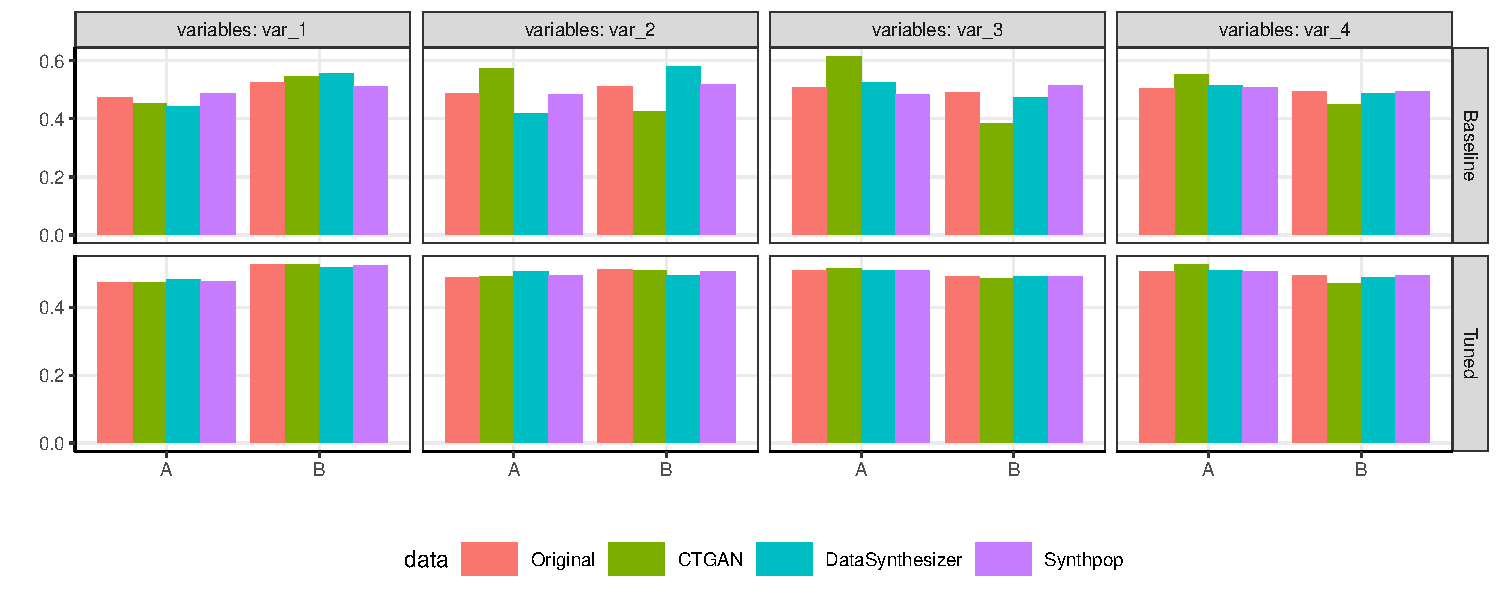
\includegraphics{../../simulation_data/categorical/graphs/graph_compare_frequency.pdf}}
    \label{graph_compare_frequency_categorical}
\end{figure}
}

\frame{\frametitle{Compare regression output between baseline and tuned}
\vspace{-5mm}
\begin{figure}
    \caption{}
    \resizebox{\textwidth}{!}{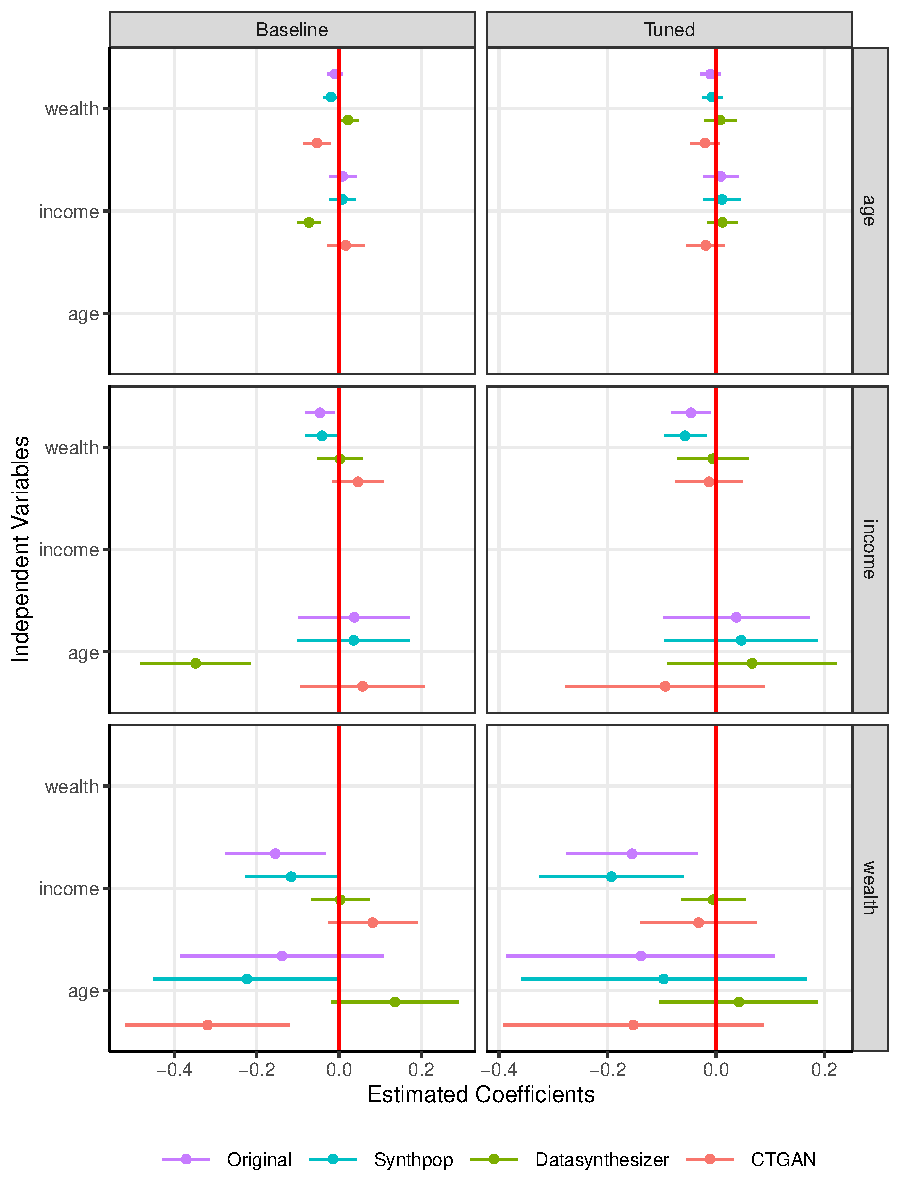
\includegraphics{../../simulation_data/categorical/graphs/graph_compare_cio_regressions.pdf}}
    \label{graph_compare_cio_regressions_categorical}
\end{figure}
}


\frame{\frametitle{Measuring utility for simulated categorical data}
\vspace{-5mm}
\begin{figure}
    \caption{}
    \resizebox{\textwidth}{!}{\includegraphics{../../simulation_data/categorical/graphs/graph_compare_utility.pdf}}
    \label{graph_compare_utility_sim_categorical}
\end{figure}
}

\frame{\frametitle{Summary: Synthpop has highest utility}
\begin{table}[h]
\caption{Comparison of Results}
\label{table_comparison}
\centering
\begin{tabular}{lrrrr}
\toprule
Data                            & ROE univar & ROE bivar & Std. Diff & CIO \\
\midrule
Simulated categorical variables & =          & =         & SP        & SP \\
\bottomrule
\end{tabular}
\end{table}
\begin{itemize}
    \item CTGAN/Datasynthesizer requires tuning (not Synthpop)
    \item Unexpectedly, CTGAN performs 2nd best for categorical data
\end{itemize}
}


\subsection{Simulated continuous data}\label{sec_results_continuous}
\frame[c]{\frametitle{}
\centering
Section \ref{sec_results}: Results \\
Section \ref{sec_results}\ref{sec_results_continuous}: Simulated continuous data
}

\frame{\frametitle{Descriptive statistics - continuous variables}
\begin{table}[!h]
    \caption{}
    \centering
    \resizebox{\textwidth}{!}{\begin{tabular}{rlrrrrr}
\toprule
number & variable & min & max & mean & std & median \\
\midrule
1 & age & 16.00 & 94.00 & 55.65 & 22.56 & 57.00 \\
2 & income & 624.00 & 349355.00 & 35721.10 & 41455.86 & 22421.50 \\
3 & wealth & -19560.00 & 89975356.00 & 659520.71 & 3165853.95 & 127616.00 \\
\bottomrule
\end{tabular}
}
    \label{table_variables_continuous}
\end{table}
}

\frame{\frametitle{Measuring utility for simulated continuous data}
\vspace{-5mm}
\begin{figure}
    \caption{}
    \resizebox{\textwidth}{!}{\includegraphics{../../simulation_data/continuous/graphs/graph_compare_utility.pdf}}
    \label{graph_compare_utility_sim_continuous}
\end{figure}
}

\frame{\frametitle{Summary: Synthpop has highest levels of utility}
\begin{table}[h]
\caption{Comparison of Results}
\label{table_comparison}
\centering
\begin{tabular}{lrrrr}
\toprule
Data                            & ROE univar & ROE bivar & Std. Diff & CIO \\
\midrule
Simulated continuous variables  & SP         & =         & SP        & SP \\
\bottomrule
\end{tabular}
\end{table}
\begin{itemize}
    \item CTGAN has similar level of CIO but higher Std. Diff
\end{itemize}
}


\subsection{UK 1991}\label{sec_results_UK1991}
\frame[c]{\frametitle{}
\centering
Section \ref{sec_results}: Results \\
Section \ref{sec_results}\ref{sec_results_UK1991}: Individual Sample of Anonymised Records (SAR) for the British Census, subsetted on the region of West Midlands (UK 1991)
}

\frame{\frametitle{Descriptive statistics - UK 1991}
\vspace{-5mm}
\begin{figure}
    \caption{}
    \vspace{-5mm}
    \resizebox{\textwidth}{!}{\includegraphics{../../UK1991/graphs/graph_descriptives.pdf}}
    \label{graph_descriptives}
\end{figure}
}

\frame{\frametitle{Measuring utility}
\vspace{-5mm}
\begin{figure}
    \caption{Ratio of estimates}
    \resizebox{\textwidth}{!}{\includegraphics{../../UK1991/graphs/graph_compare_utility_roe.pdf}}
    \label{graph_compare_utility_roe}
\end{figure}
}

\frame{\frametitle{Measuring utility}
\vspace{-5mm}
\begin{figure}
    \caption{Confidence interval overlap}
\vspace{-5mm}
    \resizebox{\textwidth}{!}{\includegraphics{../../UK1991/graphs/graph_compare_utility_cio.pdf}}
    \label{graph_compare_utility_cio}
\end{figure}
}

\frame{\frametitle{Comparing duration to create 1 synthetic data set ($\times5$)}
\begin{table}[!h]
    \caption{UK 1991 data, 12 variables (1 continuous), and  $\approx$ 20.000 observations}
    \centering
    \input{../../UK1991/tables/duration/table_duration.tex}
    \label{table_dution_UK1991}
\end{table}
}

\frame{\frametitle{Summary: things become more complicated in `real' data}
\begin{table}[h]
\caption{Comparison of Results}
\label{table_comparison}
\centering
\begin{tabular}{lrrrr}
\toprule
Data                            & ROE univar & ROE bivar & Std. Diff & CIO \\
\midrule
UK1991                          & DS/SP   & DS/SP        &           & \\
\hskip 5mm DV: MSTATUS          &            &           & CTGAN     & CTGAN \\
\hskip 5mm DV: TENURE           &            &           & SP        & SP \\
\bottomrule
\end{tabular}
\end{table}

}

\section{Conclusion}\label{sec_conclusion}
\frame[c]{\frametitle{}
\centering
Section \ref{sec_conclusion}: Conclusion
}

\frame{\frametitle{Summary}
\begin{table}[h]
\caption{Comparison of Results}
\label{table_comparison}
\centering
\begin{tabular}{lrrrr}
\toprule
Data                            & ROE univar & ROE bivar & Std. Diff & CIO \\
\midrule
Simulated categorical variables & =          & =         & SP        & SP \\
Simulated continuous variables  & SP         & =         & SP        & SP \\
UK1991                          & DS/SP   & DS/SP        &           & \\
\hskip 5mm DV: MSTATUS          &            &           & CTGAN     & CTGAN \\
\hskip 5mm DV: TENURE           &            &           & SP        & SP \\
\bottomrule
\end{tabular}
\end{table}
}



\frame{\frametitle{Summary of results}
\begin{itemize}
    \item Results a reflection of low dimensional data and focus on data utility
    \item Main message: Synthpop is the `winner'
    \begin{itemize}
        \item However, it is not always the `best'
        \item Easy - little tuning required 
        \item Fastest (data dimensionality)
        \item No privacy protection$^\dagger$
    \end{itemize}
    \item Datasynthesizer/CTGAN
    \begin{itemize}
        \item Requires tuning
    \end{itemize}
    \item CTGAN
    \begin{itemize}
        \item Slowest
    \end{itemize}
\end{itemize}
}

\frame{\frametitle{Questions}
\begin{itemize}
    \item Where is Synthpop not right?
    \item Where is CTGAN right?  Is it worth it?
    \item What are the right utility measures to use and when do we use them?
\end{itemize}
}

\frame{\frametitle{Next steps}
\begin{itemize}
    \item Privacy protection
    \item High dimensional data
    \item Assumption is that CTGAN/Datasynthesizer will perform better
\end{itemize}
}


\frame[c]{\frametitle{}
\centering
Thank you
}


\end{spacing}

\end{document}

